\documentclass[12pt,a4paper]{article}

\usepackage[margin=1in]{geometry}
\usepackage{setspace}
\usepackage{graphicx}
\usepackage{listings}
\usepackage{xcolor}
\usepackage{hyperref}
\usepackage{booktabs}
\usepackage{array}
\usepackage{float}

\onehalfspacing

\definecolor{codegray}{rgb}{0.5,0.5,0.5}
\definecolor{codeblue}{rgb}{0.13,0.13,0.55}
\definecolor{boxgray}{rgb}{0.93,0.93,0.93}

\lstset{
    basicstyle=\ttfamily\small,
    keywordstyle=\color{codeblue},
    commentstyle=\color{codegray},
    frame=single,
    breaklines=true,
    showstringspaces=false
}

% A simple shaded definition box
\newcommand{\defbox}[2]{%
  \vspace{0.2cm}
  \noindent\colorbox{boxgray}{\parbox{\dimexpr\linewidth-2\fboxsep}{%
    \textbf{#1:} #2
  }}
  \vspace{0.2cm}
}

\begin{document}

% ─────────────────────────────────────────────
%  Header
% ─────────────────────────────────────────────
\begin{center}
    {\Large \textbf{CSE312: Database Management Systems Lab}}\\[0.3cm]
    {\large \textbf{Lab 01: Entity–Relationship (ER) Diagram Using draw.io}}
\end{center}

\vspace{0.5cm}

% ─────────────────────────────────────────────
%  1. Objective
% ─────────────────────────────────────────────
\section*{1. Objective}
The objectives of this experiment are:
\begin{itemize}
    \item To understand the fundamental concepts of the Entity–Relationship (ER) model.
    \item To identify entities, attributes, and relationships in a real-world scenario.
    \item To construct an ER diagram using the draw.io diagramming tool.
    \item To represent weak entities, participation constraints, and various attribute types in an ER diagram.
\end{itemize}

% ─────────────────────────────────────────────
%  2. Introduction
% ─────────────────────────────────────────────
\section*{2. Introduction}
The Entity–Relationship (ER) model is a high-level conceptual data model used in the design of databases.
It provides a graphical representation of the logical structure of a database, making it easier for
designers and stakeholders to understand data requirements before implementation.

\textbf{draw.io} (also known as \texttt{diagrams.net}) is a free, browser-based diagramming tool that
supports the creation of ER diagrams, flowcharts, UML diagrams, and more.
It requires no installation and allows diagrams to be exported in various formats (PNG, SVG, PDF, XML).

\noindent\textbf{Accessing draw.io:}
\begin{itemize}
    \item Open a web browser and navigate to \url{https://app.diagrams.net}.
    \item Choose a storage location (Device, Google Drive, GitHub, etc.) or select \textit{Decide later}.
    \item Start a new blank diagram or choose the \textit{Entity Relation} template from the template gallery.
\end{itemize}

% ─────────────────────────────────────────────
%  3. Theory
% ─────────────────────────────────────────────
\section*{3. Theory}

% 3.1 Entity and Entity Type
\subsection*{3.1 Entity and Entity Type}

\defbox{Entity}{An \textbf{entity} is a real-world object or concept that has an independent existence and
can be distinctly identified. For example, a specific student \textit{Alice} or the course \textit{CSE301}
are entities.}

\defbox{Entity Type}{An \textbf{entity type} defines a collection (set) of entities that share the same
attributes and properties. It represents the \textit{schema} or blueprint for a group of similar
entities. Example: \texttt{STUDENT}, \texttt{COURSE}, \texttt{EMPLOYEE}.}

\noindent In an ER diagram, an entity type is represented by a \textbf{rectangle}.

\vspace{0.3cm}
\begin{figure}[H]
    \centering
    % ── INSERT SCREENSHOT: draw.io entity rectangle (e.g., STUDENT) ──
    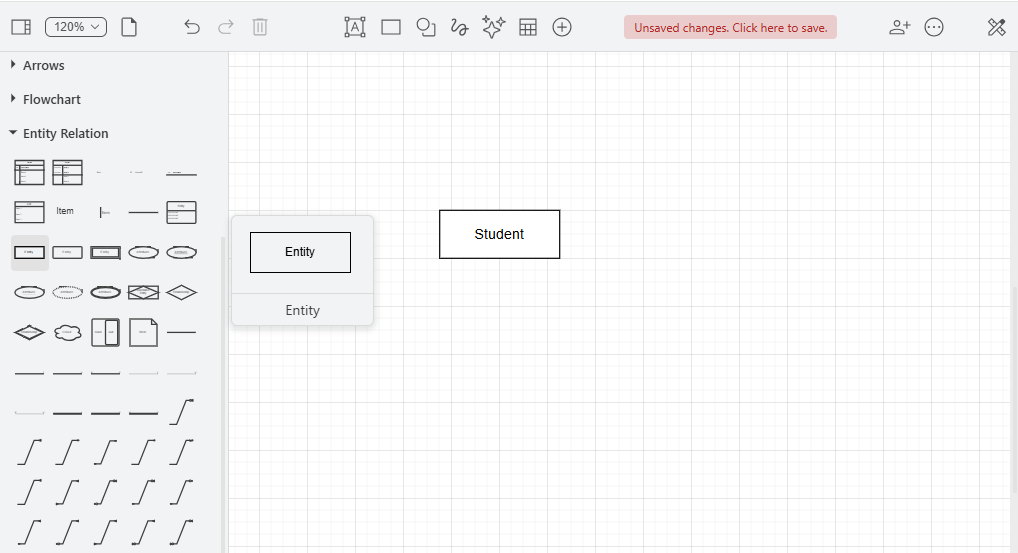
\includegraphics[width=\linewidth]{student-entity.png}
    \caption{Entity type \texttt{STUDENT} represented as a rectangle in draw.io}
    \label{fig:entity}
\end{figure}

% 3.2 Relationship and Relationship Type
\subsection*{3.2 Relationship and Relationship Type}

\defbox{Relationship}{A \textbf{relationship} is an association among two or more entities.
For example, the fact that student \textit{Alice} is \textit{enrolled in} course \textit{CSE301}
is a relationship instance.}

\defbox{Relationship Type}{A \textbf{relationship type} defines a set of associations among entity
types. It has a name and specifies which entity types participate in it.
Example: \texttt{ENROLLS\_IN} between \texttt{STUDENT} and \texttt{COURSE}.}

\noindent In an ER diagram, a relationship type is represented by a \textbf{diamond} connected to
the participating entity rectangles by lines.

The \textbf{degree} of a relationship is the number of participating entity types:
\begin{itemize}
    \item \textbf{Binary} -- two entity types (most common).
    \item \textbf{Ternary} -- three entity types.
    \item \textbf{Unary (Recursive)} -- one entity type related to itself.
\end{itemize}

\vspace{0.3cm}
\begin{figure}[H]
    \centering
    % ── INSERT SCREENSHOT: STUDENT ─ ENROLLS_IN ─ COURSE diamond in draw.io ──
    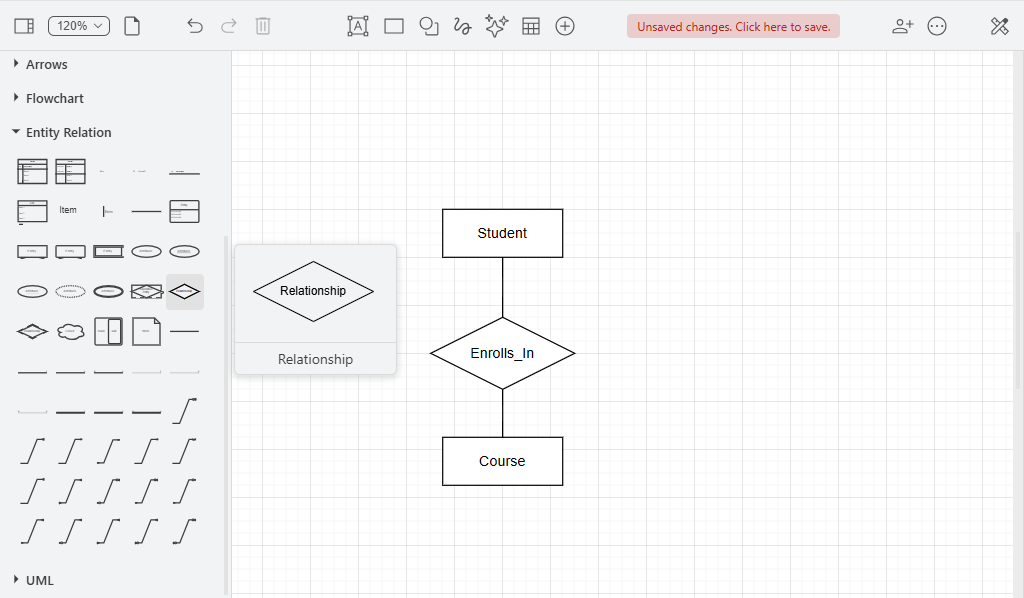
\includegraphics[width=1\linewidth]{enrolls_in_relationship.png}
    \caption{Relationship type \texttt{ENROLLS\_IN} between \texttt{STUDENT} and \texttt{COURSE}}
    \label{fig:relationship}
\end{figure}

Cardinality of a relationship is the number of relationship instances each entity participates in. The cardinality of a relationship can be of the following types:
\begin{itemize}
    \item \textbf{One-to-One (1:1)} -- One entity of each side can form relationship with at most one other entity.
    \item \textbf{One-to-Many (1:M)} -- Entities from \textit{One} side can form relationship with more than one entities from \textit{Many} side.
    \item \textbf{Many7-to-Many (M:M)} -- Entities from both sides can form relationship with more than one entities from the other side.
\end{itemize}

\vspace{0.3cm}
\begin{figure}[H]
    \centering
    % ── INSERT SCREENSHOT: cardinality types in draw.io ──
    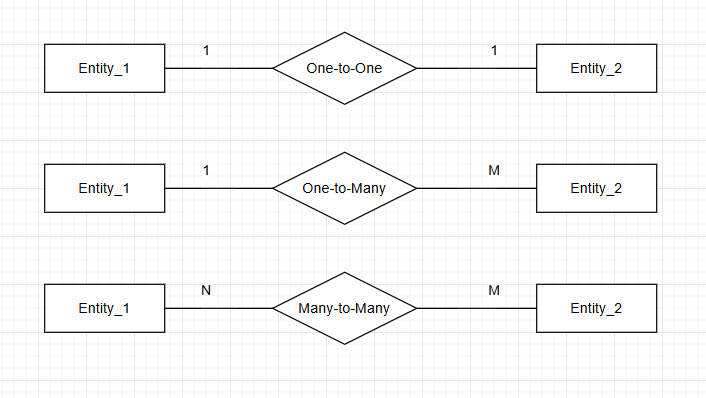
\includegraphics[width=0.75\linewidth]{cardinalities.png}
    \caption{Different cardinalities in draw.io}
    \label{fig:cardinalities}
\end{figure}

% 3.3 Attributes and Their Types
\subsection*{3.3 Attributes and Their Types}

\defbox{Attribute}{An \textbf{attribute} is a property or characteristic that describes an entity type
or a relationship type. Example: \texttt{Name}, \texttt{Age}, and \texttt{StudentID} are attributes
of \texttt{STUDENT}.}

\noindent The following attribute types are commonly used in ER diagrams:

\vspace{0.2cm}
\begin{table}[H]
\centering
\renewcommand{\arraystretch}{1.4}
\begin{tabular}{>{\bfseries}p{3.5cm} p{6.5cm} p{3.5cm}}
\toprule
Attribute Type & Description & ER Notation \\
\midrule
Simple (Atomic) & Cannot be divided further. \newline e.g., \texttt{Age}, \texttt{Gender} & Oval \\
Composite & Can be divided into sub-parts. \newline e.g., \texttt{Name} → First, Last & Oval with child ovals \\
Multi-valued & Can hold multiple values. \newline e.g., \texttt{PhoneNumbers} & Double oval \\
Derived & Computed from another attribute. \newline e.g., \texttt{Age} from \texttt{DOB} & Dashed oval \\
Key & Uniquely identifies each entity. \newline e.g., \texttt{StudentID} & Oval with underlined text \\
\bottomrule
\end{tabular}
\caption{Types of attributes and their ER diagram notation}
\label{tab:attributes}
\end{table}

\vspace{0.3cm}
\begin{figure}[H]
    \centering
    % ── INSERT SCREENSHOT: attribute types on STUDENT entity in draw.io ──
    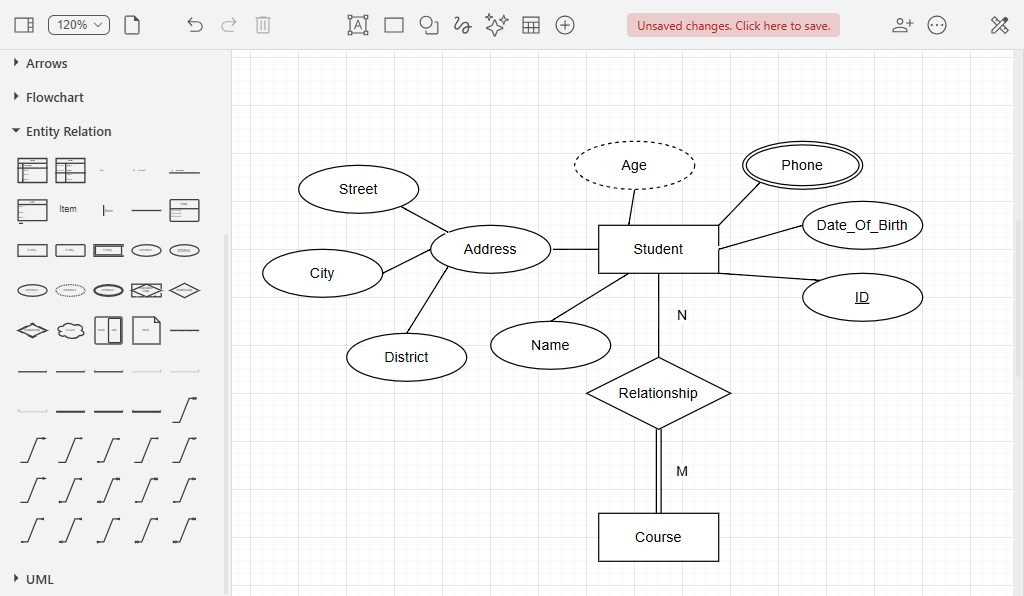
\includegraphics[width=1\linewidth]{student_entity_attributes.png}
    \caption{Different attribute types connected to the \texttt{STUDENT} entity in draw.io}
    \label{fig:attributes}
\end{figure}

% 3.4 Weak Entities
\subsection*{3.4 Weak Entities}

\defbox{Weak Entity Type}{A \textbf{weak entity type} is an entity type that does not have a key
attribute of its own. It depends on another entity type (the \textbf{owner} or \textbf{strong} entity)
for its identification. Example: \texttt{DEPENDENT} (of an employee) depends on \texttt{EMPLOYEE}.}

\noindent Key characteristics of weak entities:
\begin{itemize}
    \item Represented by a \textbf{double rectangle}.
    \item The relationship connecting it to its owner is called an \textbf{identifying relationship},
          represented by a \textbf{double diamond}.
    \item A weak entity has a \textbf{partial key} (discriminator), underlined with a \textit{dashed} line,
          that uniquely identifies it \textit{within} the owner's context.
    \item A weak entity always has a \textbf{total participation} constraint with its identifying relationship.
\end{itemize}

\vspace{0.3cm}
\begin{figure}[H]
    \centering
    % ── INSERT SCREENSHOT: EMPLOYEE ══ HAS ══ DEPENDENT (double rectangle and diamond) ──
    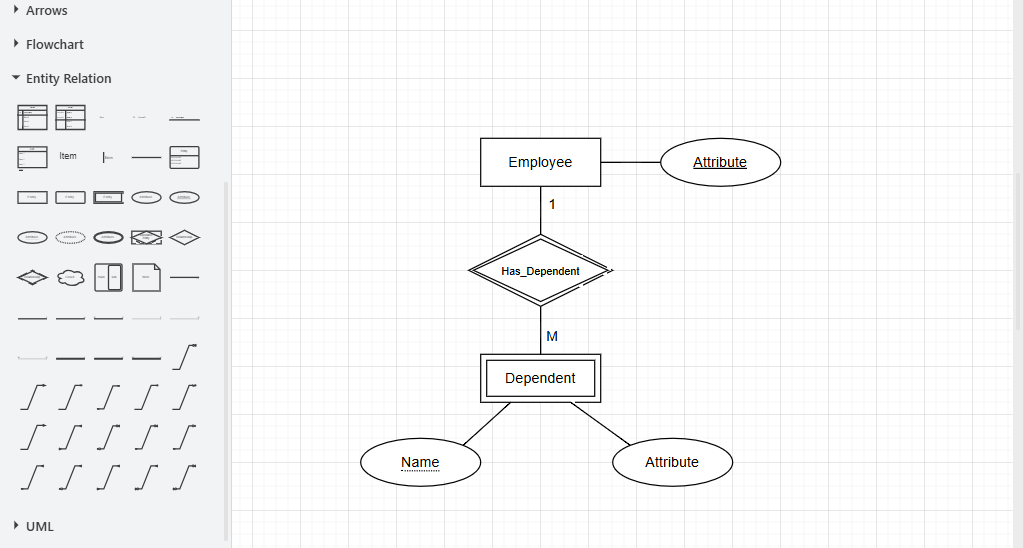
\includegraphics[width=1\linewidth]{employee-dependent-identifying-relationship.png}
    \caption{\texttt{DEPENDENT} as a weak entity of \texttt{EMPLOYEE} in draw.io}
    \label{fig:weak_entity}
\end{figure}

% 3.5 Participation Constraints
\subsection*{3.5 Participation Constraints}

\defbox{Participation Constraint}{A \textbf{participation constraint} specifies whether the existence
of an entity depends on it being related to another entity through a relationship.}

\noindent There are two types:

\begin{itemize}
    \item \textbf{Total Participation (Mandatory):} Every entity in the entity type \textit{must}
          participate in at least one relationship instance. Denoted by a \textbf{double line} between
          the entity rectangle and the relationship diamond.
          \textit{Example:} Every \texttt{EMPLOYEE} must work for a \texttt{DEPARTMENT}.

    \item \textbf{Partial Participation (Optional):} Some entities may not participate in any
          relationship instance. Denoted by a \textbf{single line}.
          \textit{Example:} Not every \texttt{EMPLOYEE} manages a \texttt{DEPARTMENT}.
\end{itemize}

\vspace{0.3cm}
\begin{figure}[H]
    \centering
    % ── INSERT SCREENSHOT: EMPLOYEE ══ WORKS_FOR ─ DEPARTMENT showing participation ──
    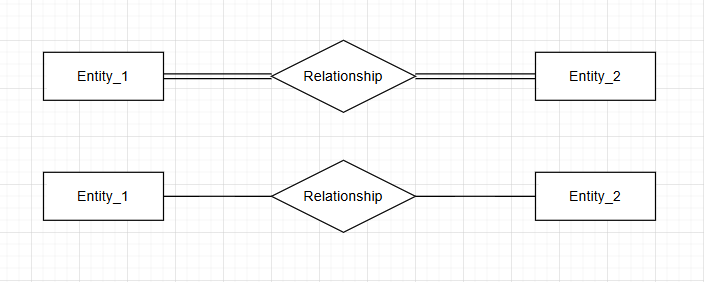
\includegraphics[width=0.7\linewidth]{total-and-partial-relationship.png}
    \caption{Total (double line) and partial (single line) participation in draw.io}
    \label{fig:participation}
\end{figure}

% ─────────────────────────────────────────────
%  4. Procedure
% ─────────────────────────────────────────────
\section*{4. Procedure}

\subsection*{4.1 Opening draw.io and Selecting the ER Template}
\begin{enumerate}
    \item Open a browser and navigate to \url{https://app.diagrams.net}.
    \item In the Shapes section, expand the \textbf{Entity Relation} template.
\end{enumerate}

\subsection*{4.2 Adding Entities}
\begin{enumerate}
    \item From the left panel under \textit{Entity Relation}, drag a \textbf{Entity} shape (rectangle)
          onto the canvas.
    \item Double-click the shape to rename it (e.g., \texttt{STUDENT}).
    \item For a \textbf{weak entity}, use the double-bordered rectangle shape.
\end{enumerate}

\subsection*{4.3 Adding Attributes}
\begin{enumerate}
    \item Drag an \textbf{Attribute} shape (oval/ellipse) onto the canvas near the entity.
    \item Double-click and name it (e.g., \texttt{StudentID}).
    \item Connect it to the entity using the \textbf{connector} tool (hover over the entity border
          until a blue arrow appears, then drag to the attribute oval).
    \item For a \textbf{key attribute}, underline the text: right-click the shape $\to$ \textit{Edit Style}
          $\to$ add \texttt{fontStyle=4;} (value 4 = underline).
    \item For a \textbf{multi-valued attribute}, use a double-bordered oval.
    \item For a \textbf{derived attribute}, use a dashed-bordered oval: \texttt{dashed=1;}.
\end{enumerate}

\subsection*{4.4 Adding Relationships}
\begin{enumerate}
    \item Drag a \textbf{Relationship} shape (diamond) onto the canvas between two entities.
    \item Double-click and name it (e.g., \texttt{ENROLLS\_IN}).
    \item Connect the diamond to each participating entity using connectors.
    \item Add \textbf{cardinality labels} (1, N, M) on the connector lines near each entity.
    \item For an \textbf{identifying relationship} (weak entity), use a double-bordered diamond.
\end{enumerate}

\subsection*{4.5 Setting Participation Constraints}
\begin{enumerate}
    \item Select the connector between an entity and a relationship diamond.
    \item Right-click $\to$ \textit{Edit Style}.
    \item For \textbf{total participation}, change the line style to \texttt{strokeWidth=3;} or add a
          double-line by setting \texttt{endFill=1;} with a parallel line effect.
    \item For \textbf{partial participation}, keep the default single-line connector.
\end{enumerate}

\subsection*{4.6 Exporting the Diagram}
\begin{enumerate}
    \item Go to \textbf{File} $\to$ \textbf{Export As}.
    \item Select \textbf{PNG} or \textbf{PDF} for submission.
    \item Save the XML source via \textbf{File} $\to$ \textbf{Save} for future editing.
\end{enumerate}

% \vspace{0.3cm}
% \begin{figure}[H]
%     \centering
%     % ── INSERT SCREENSHOT: complete ER diagram in draw.io canvas ──
%     \fbox{\rule{0pt}{6cm}\hspace{11cm}}
%     \caption{Complete ER diagram of the sample scenario in draw.io}
%     \label{fig:complete_er}
% \end{figure}

% ─────────────────────────────────────────────
%  5. Observations
% ─────────────────────────────────────────────
\section*{5. Observations}
\begin{itemize}
    \item Entity types were successfully represented using rectangles and named appropriately.
    \item Attributes of various types (simple, composite, multi-valued, derived, key) were attached
          to entities using the correct ER notation.
    \item Relationships were modelled using diamonds with cardinality labels (1:1, 1:N, M:N).
    \item Weak entities and their identifying relationships were distinguished using double-bordered
          shapes.
    \item Participation constraints were indicated using single and double connector lines.
\end{itemize}

% ─────────────────────────────────────────────
%  6. Lab Task
% ─────────────────────────────────────────────
\section*{6. Lab Task}
\subsection*{Task A: University Management System (Guided)} 
Design an ER diagram for a \textbf{University Management System} with the following requirements:

\begin{enumerate}
    \item \textbf{Entities:} \texttt{STUDENT}, \texttt{FACULTY}, \texttt{DEPARTMENT}, \texttt{COURSE}.
    \item \textbf{Attributes:}
    \begin{itemize}
        \item \texttt{STUDENT}: \texttt{StudentID} (key), \texttt{Name} (composite: First, Last),
              \texttt{PhoneNumbers} (multi-valued), \texttt{Age} (derived from DOB).
        \item \texttt{COURSE}: \texttt{CourseCode} (key), \texttt{Title}, \texttt{Credits}.
        \item \texttt{FACULTY}: \texttt{FacultyID} (key), \texttt{Name}, \texttt{Designation}.
        \item \texttt{DEPARTMENT}: \texttt{DeptID} (key), \texttt{DeptName}, \texttt{Location}.
    \end{itemize}
    \item \textbf{Relationships:}
    \begin{itemize}
        \item \texttt{STUDENT} \textit{enrolls in} \texttt{COURSE} (M:N).
        \item \texttt{FACULTY} \textit{teaches} \texttt{COURSE} (1:N).
        \item \texttt{DEPARTMENT} \textit{offers} \texttt{COURSE} (1:N).
        \item \texttt{FACULTY} \textit{belongs to} \texttt{DEPARTMENT} (N:1, total participation
              for \texttt{FACULTY}).
    \end{itemize}
    \item Indicate all participation constraints appropriately.
    \item Export the completed diagram as a PNG and attach it to your lab report.
\end{enumerate}

\subsection*{Task B: Hospital Management System (Unguided)}
Imagine a hospital management system where various elements need to be modeled.

In this system, there are components such as "Patient," "Doctor," and "Department." The "Patient" element has characteristics like "PatientID," "Name," "Address," and "DateOfBirth." The "Doctor" element includes details such as "DoctorID," "Name," "Specialization," and "YearsOfExperience." The "Department" component has identifiers like "DepartmentID," "DepartmentName," and "Location."

Consider the element "Appointment" that represents a scheduled interaction between a patient and a doctor. This component includes specifics like "AppointmentDate," "AppointmentTime," and "ConsultationFee." The "Appointment" element is closely connected to both the "Patient" and "Doctor" components and derives its existence from these connections.

Various interactions occur in this system. For example, one interaction might indicate that a "Patient" schedules an appointment with a "Doctor," where details like "PurposeOfVisit" are recorded. Another interaction could show that a "Doctor" is associated with a "Department," indicating their work area.

\textbf{Draw} an Entity-Relationship Diagram based on the above description.

% ─────────────────────────────────────────────
%  7. Conclusion
% ─────────────────────────────────────────────
\section*{7. Conclusion}
This experiment provided a hands-on introduction to the Entity–Relationship model and its practical
application using the draw.io diagramming tool. Through identifying entities, attributes, and
relationships, and representing them with the standard ER notation, students gained foundational
skills required for conceptual database design. These skills form the basis for translating a
real-world problem into a structured relational schema in subsequent experiments.

\end{document}